\section{Results} \label{sec: res}

 As stated in \autoref{sec: stat}, the first step to obtain the system's response is to compute the number of modes per bandwidth. The modal density $n_p$ of a thin plate can be expressed as
 \begin{equation}
 n_p(\omega)=\frac{A}{4\pi}\sqrt{\frac{\rho t }{D}}
 \end{equation}
 where $\rho$ is the density, $D$ is the stiffness, $A$ is the area and $t$ the thickness. And being $n_a$ the modal density of the air layers:
 
 \begin{equation}
n_a(\omega)=\frac{V}{\pi c_0} \left(\frac{\omega}{c_0}\right)^2+\frac{A_{air}}{4 c_0}\left(\frac{\omega}{c_0}\right)+\frac{L_{air}}{8 c_0},
\end{equation}  

where $V$ is the volume of the air cavity, $A_{air}$ the area of all the faces defining this volume and $L_{air}$ perimeter defined by it.

Knowing that the number of modes in a bandwidth $\Delta f$ is 
\begin{equation}
N=n\Delta f ,
\end{equation}

the number of modes per bandwidth can be seen in \autoref{fig: modes}, where it  is easy to see that the high-frequency condition is satisfied at frequencies higher than 2000 Hz. Note that this condition is satisffied only when both, the panels and the air layers reach 5 modes per bandwidth.

\begin{figure}[H]
    \centering
    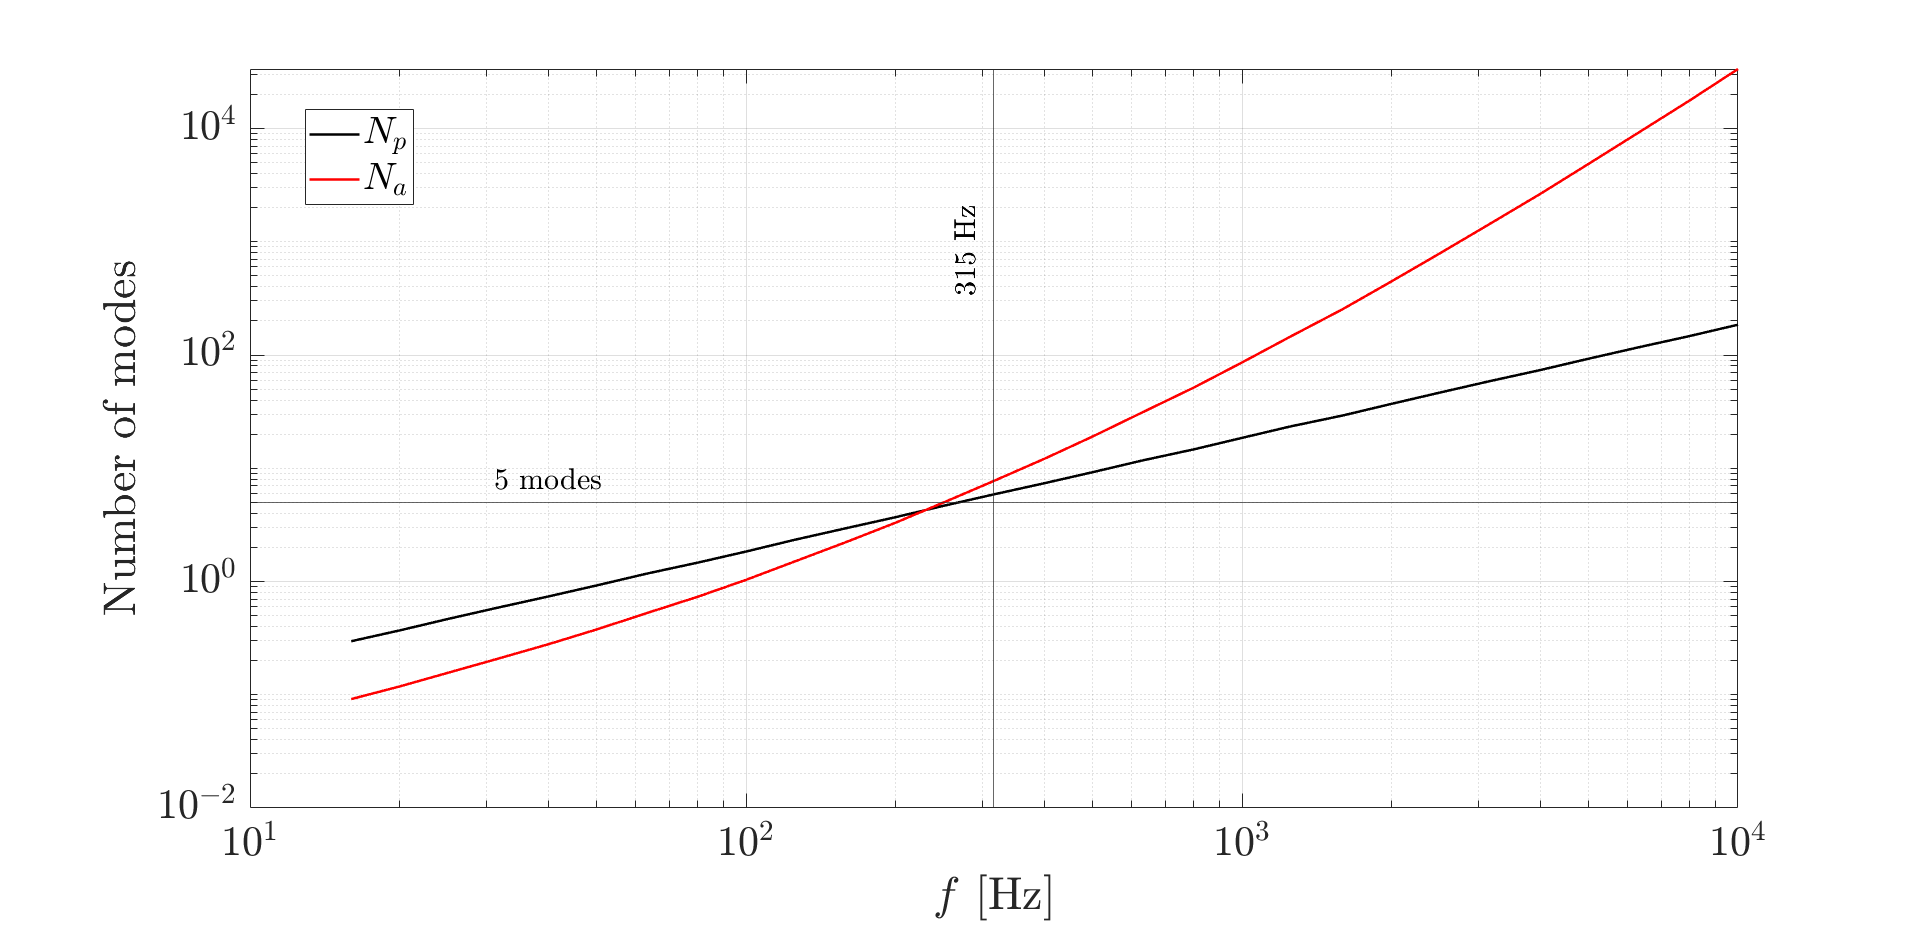
\includegraphics[width=0.9\linewidth]{Figures/modes.png}
    \caption{Number of modes per bandwidth.}
    \label{fig: modes}
\end{figure}

Once the application range of the system is defined, and with the modal densities of the different subsystems calculated, the coupling loss factors (CLF) of the system are defined based on the power radiated by the panels to the air layers, taking into account the radiation efficiency of the panels, as expressed by:

\begin{equation}
\eta_{p a}=\frac{A \rho_0 c_0 \sigma(\omega)}{M \omega},
\end{equation}
where $M$ is the mass of the panel and $\sigma$ is the radiation efficiency of the panel, expressed as
Then, $\eta_{ap}$ is obtained from the reciprocity relation expressed in \autoref{eq: reciproc}. The resulting CLF's are shown in \autoref{fig: etas}

\begin{figure}[H]
    \centering
    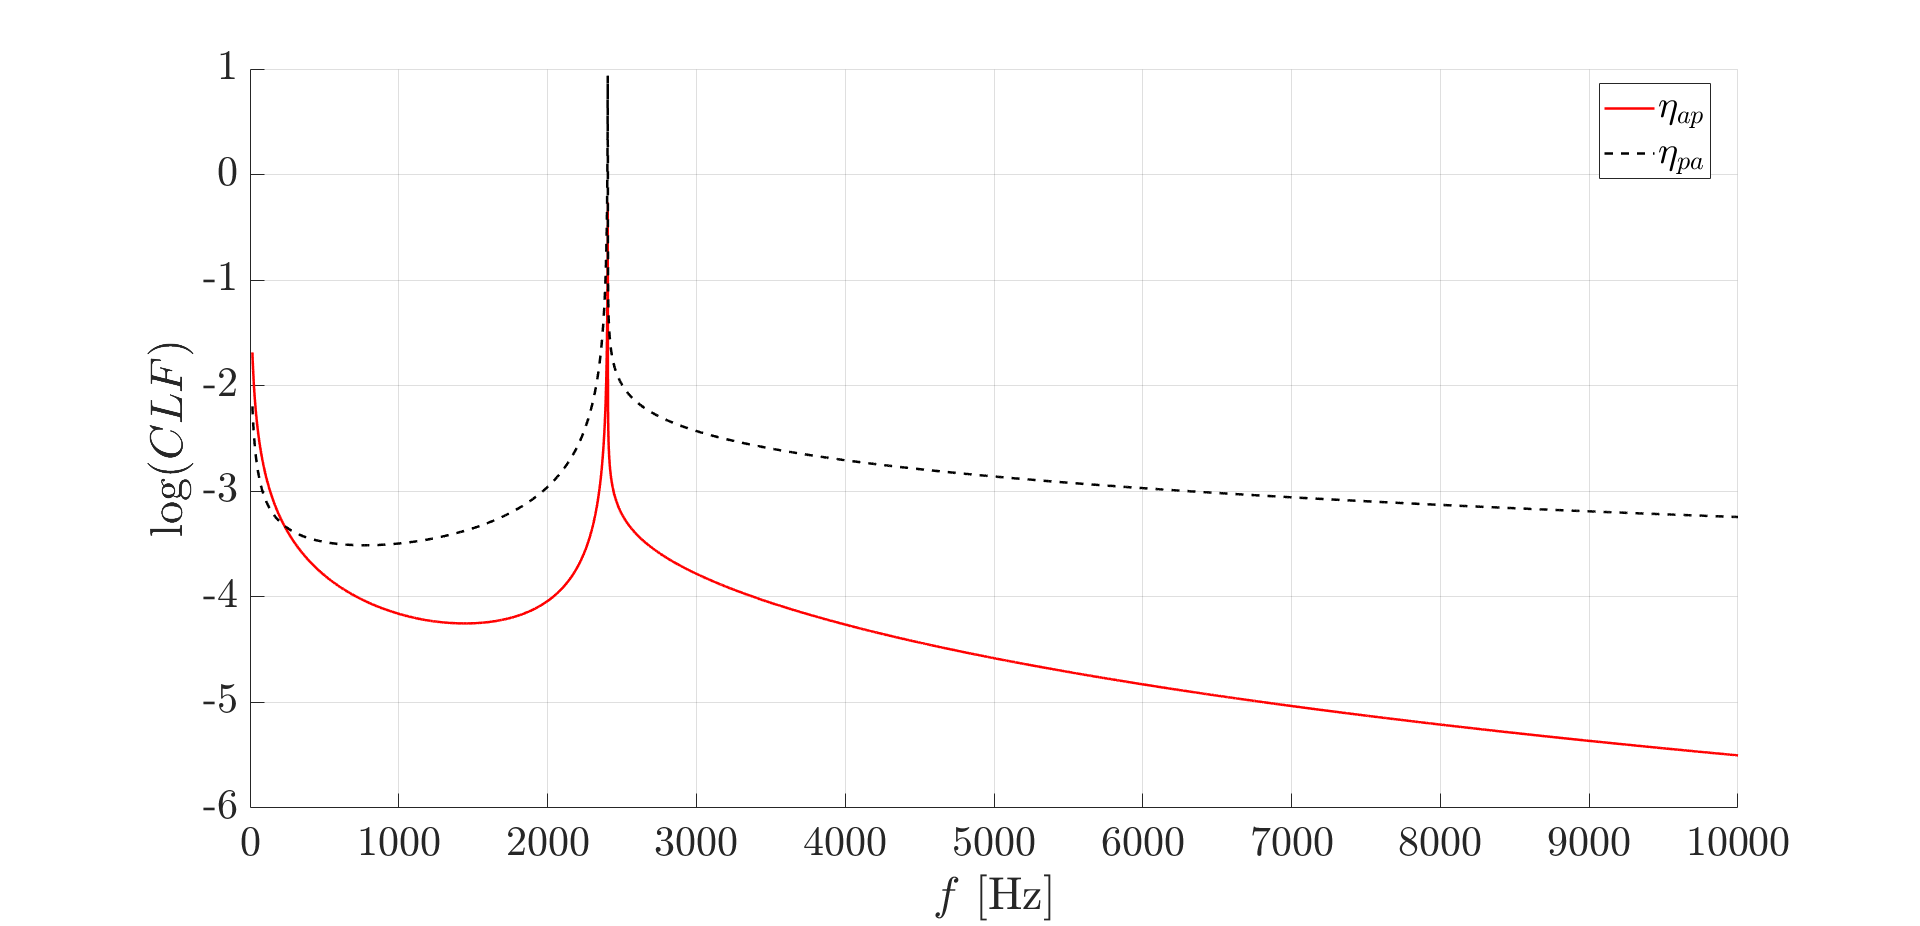
\includegraphics[width=0.9\linewidth]{Figures/etas.png}
    \caption{Coupling loss factors of the panels and the air layers.}
    \label{fig: etas}
\end{figure}

With the CLF's computed, the statistic analysis method can be implemented as shown in \autoref{eq: system}.
\begin{equation}
    \label{eq: system}
    \omega \cdot\left(\begin{array}{ccccc}
    \eta_p+\eta_{p a} & -\eta_{a p} & 0 & 0 & 0 \\
    -\eta_{p a} & \eta_a+\eta_{a p} & -\eta_{p a} & 0 & 0 \\
    0 & -\eta_{a p} & \eta_p+\eta_{p a} & -\eta_{a p} & 0 \\
    0 & 0 & -\eta_{p a} & \eta_a+\eta_{a p} & -\eta_{p a} \\
    0 & 0 & 0 & -\eta_{a p} & \eta_p+\eta_{p a}
    \end{array}\right)\left\{\begin{array}{c}
    E_1 \\
    E_2 \\
    E_3 \\
    E_4 \\
    E_5
    \end{array}\right\}=\left(\begin{array}{c}
    P_1(f) \\
    0 \\
    P_3(f) \\
    0 \\
    P_5(f)
    \end{array}\right)
\end{equation}

Isolating the energies vector in \autoref{eq: system}, the resulting energy of each subsystem can be seen in \autoref{fig: E}

\begin{figure}[H]
    \centering
    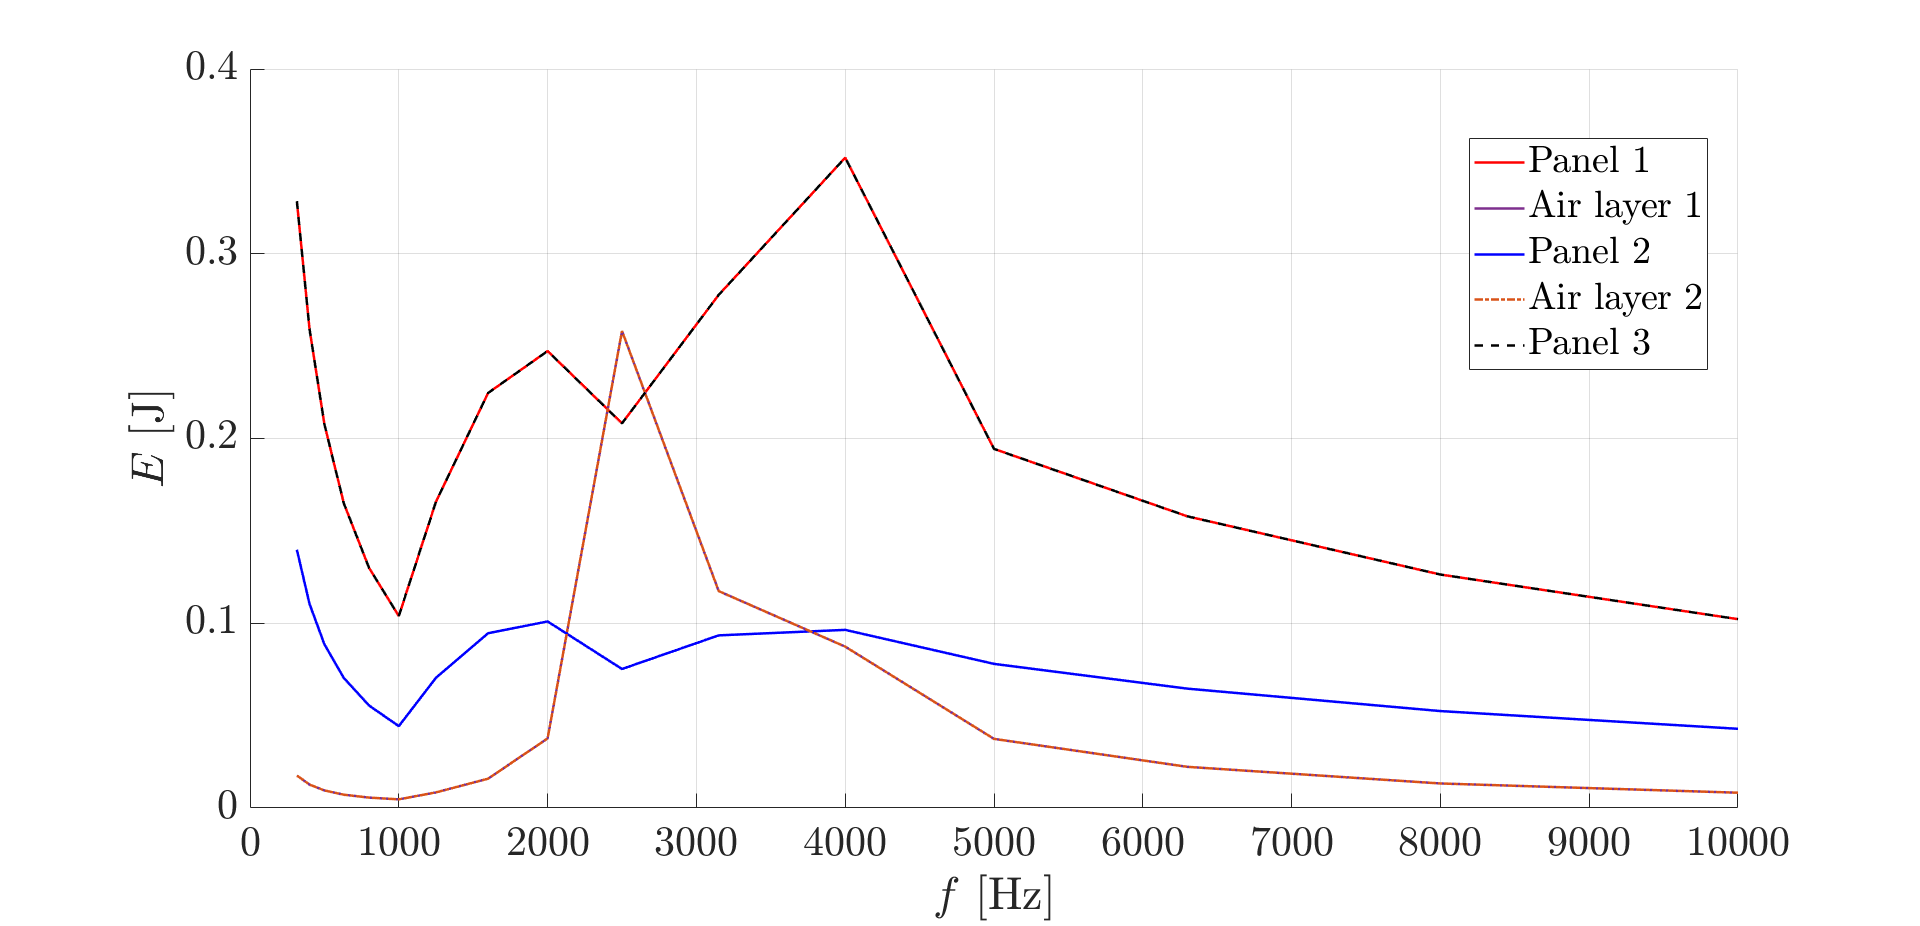
\includegraphics[width=0.9\linewidth]{Figures/E.png}
    \caption{Energy of each subsystem.}
    \label{fig: E}
\end{figure}

Knowing that the energy is related with the average velocity of the panels and with the root mean square pressure of the air  by the following relation,

\begin{equation}
    E = m v^2 = \frac{V}{\rho_0 c_0^2} P^2,
\end{equation}

the response of each subsystem is shown in Figures \ref{fig: pRMS} and \ref{fig: vRMS}
\begin{figure}[H]
    \centering
    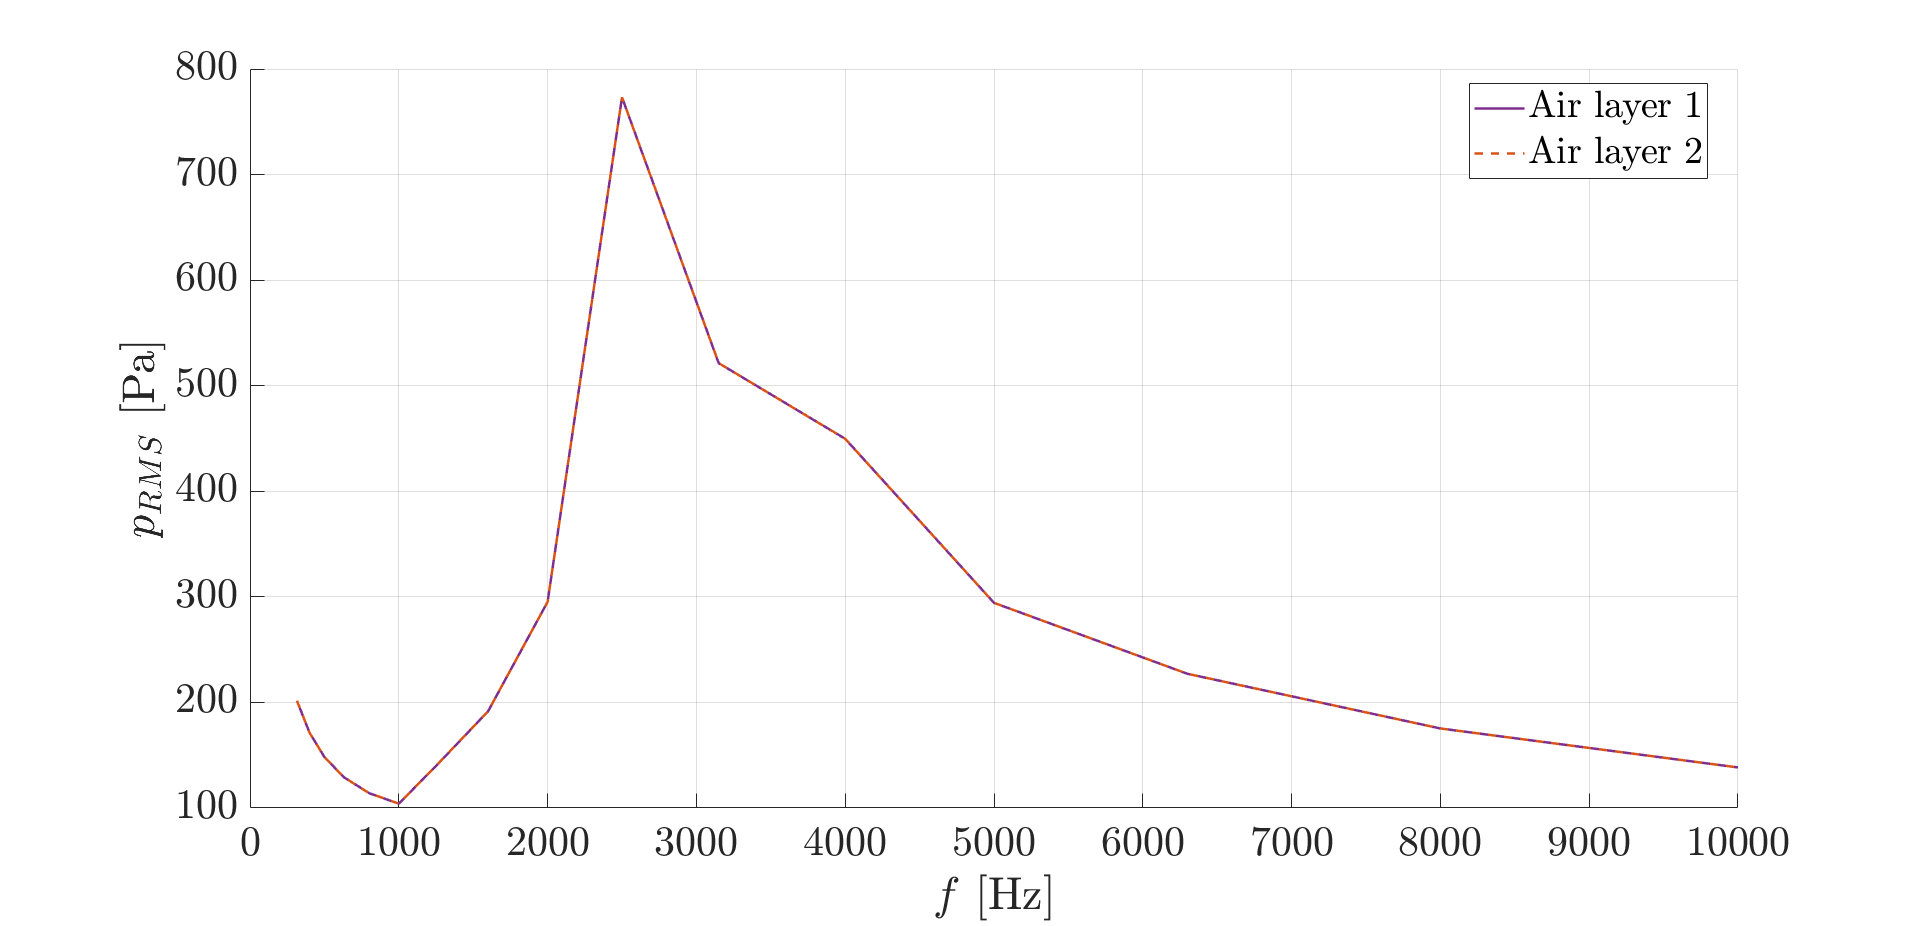
\includegraphics[width=0.9\linewidth]{Figures/pRMS.png}
    \caption{RMS pressure of the air in each air layer.}
    \label{fig: pRMS}
\end{figure}
\begin{figure}[H]
    \centering
    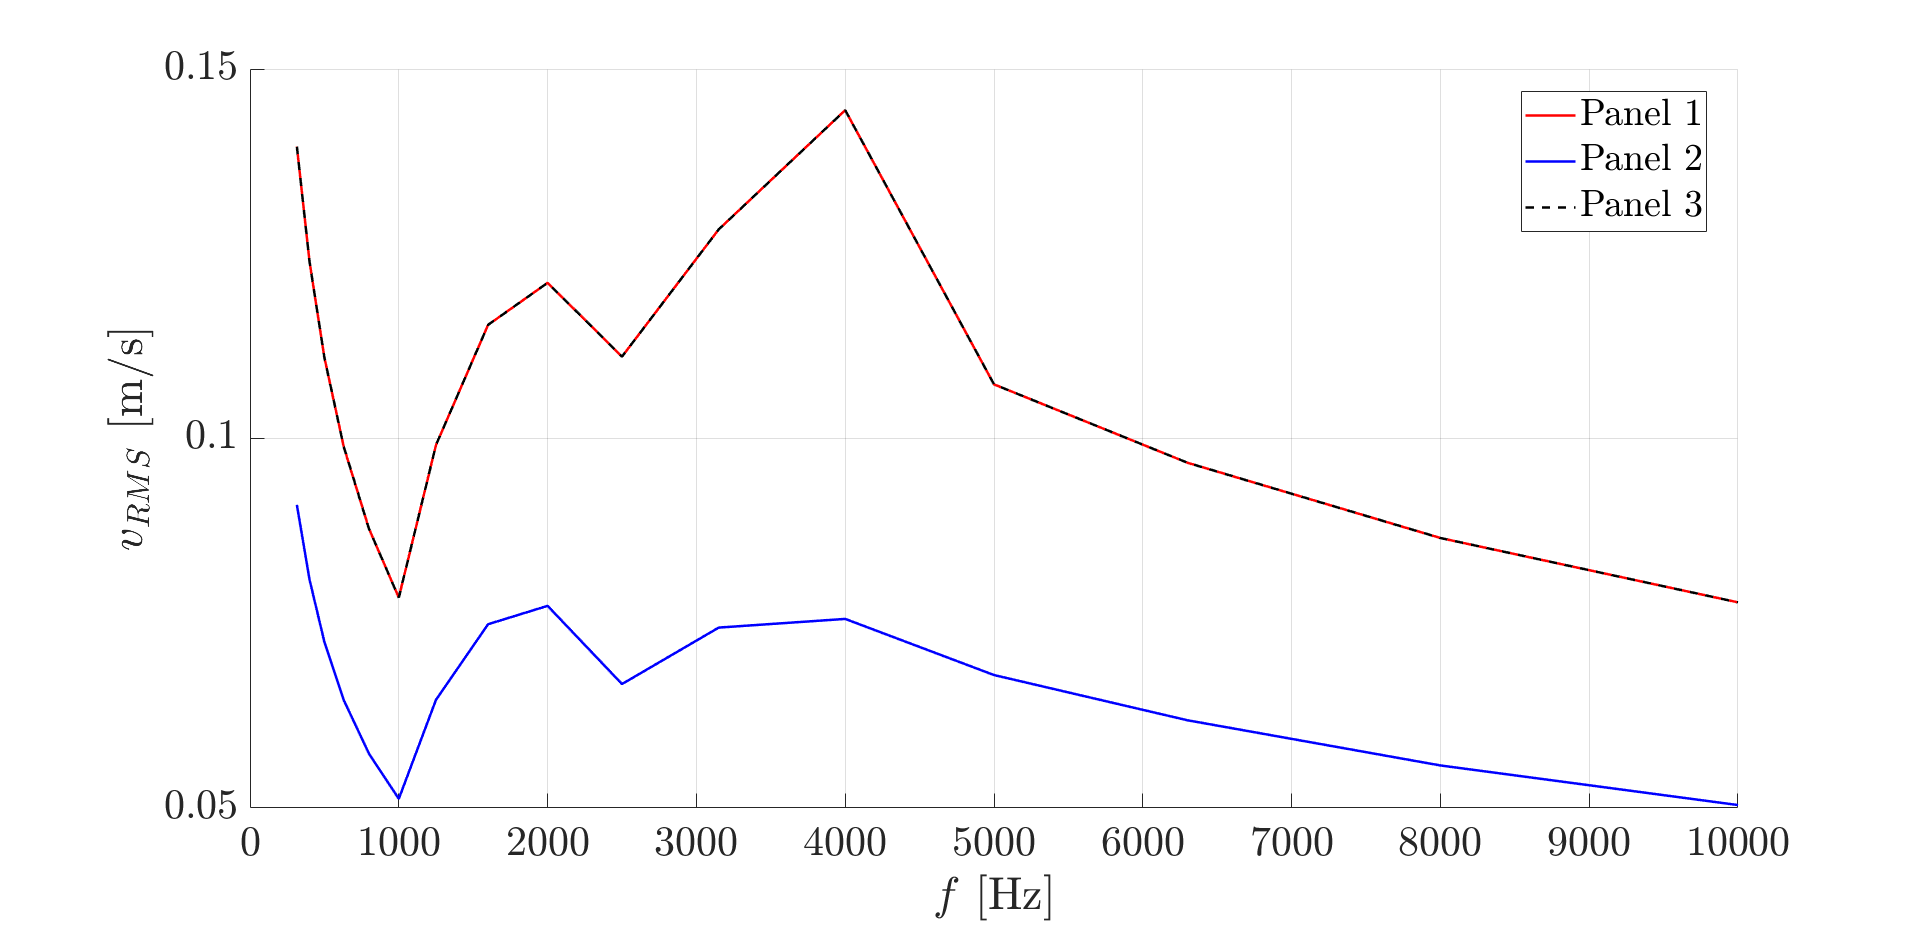
\includegraphics[width=0.9\linewidth]{Figures/vRMS.png}
    \caption{Average velocity of each panel.}
    \label{fig: vRMS}
\end{figure}

Note that as the complete system is symmetric, the responses of the first and third panel, and the responses of the two are layers are exactly the same. Therefore, the central panel's response seems to be damped by the symmetrical response of the rest of subsystems. 
